\section{Description and Methodology}

\subsection{Linux build process}
To build the uCLinux distribution for the microcontroller, PTXDist is
used\cite{ptxdistguru}. This is done because the features of a real
distrobution is wanted, and PTXDist allows to create a unique distrobution.

\begin{verbatim}
ptxdist select configs/ptxconfig
ptxdist platform <platform>
ptxdist toolchain <toolchain>
\end{verbatim}

\noindent
These commands are run to set the userland configuration, which platform to
develop for and choosing the toolchain to build for this platform

\begin{verbatim}
ptxdist go
\end{verbatim}

\noindent
Is used to compile the components needed. The script is smart enough to not
compile everything everytime it is runned, so it can be used to just compile
some parts of the project.

\begin{verbatim}
ptxdist images
\end{verbatim}

\noindent
To build the image that can be flashed to the device, this command is used. To
not build the root image every time other parts of the distrobution is edited,
the specific image to build can be used.

\begin{verbatim}
ptxdist test flash-all
\end{verbatim}

\noindent
This is used to flash all images to the device. Again, to not flash things that
don't need to be flashed each time, a more specific image to flash can be given
as argument.


\subsection{The driver}

To receive button inputs from the player, a driver for the
provided gamepad was implemented. Because the gamepad isn't discoverable, it is
implemented as a platform device. This means that the platform driver
\footnotemark registers that it can handle the device "tdt4259", which is then
matched by the system to the platform device by the same name.

\footnotetext{
  \url{https://www.kernel.org/doc/Documentation/driver-model/platform.txt}
}

As opposed to the old way of implementing drivers in Linux, when the module is
loaded or unloaded, it is merely registered or unregistered as an available
platform driver. The system will then call the registered probe() and release()
functions when required.

\begin{algorithmic}
  \footnotesize
  \Function{dev\_probe}{pdev}
    \State $\Call{hardware\_init}{\null}$ \\

    \State $irq\_even \gets \Call{platform\_get\_irq}{pdev, irq\_even}$
    \State $irq\_odd \gets \Call{platform\_get\_irq}{pdev, irq\_odd}$
    \State $\Call{request\_irq}{irq\_even, irq\_handler\_func, \
      irqf\_disabled, device\_name, null}$
    \State $\Call{request\_irq}{irq\_odd, irq\_handler\_func, \
      irqf\_disabled, device\_name, null}$ \\

    \State $res \gets \Call{platform\_get\_resource}{pdev, ioresource\_mem, 0}$
    \State $size \gets \Call{resource\_size}{res}$
    \State $\Call{request\_mem\_region}{res.start,  size, \
      pdev{\rightarrow}name}$ \\

    \State $\Call{alloc\_chrdev\_region}{\&devno, 0, 1, device\_name}$ \\


    \State $cl \gets \Call{class\_create}{this\_module, device\_name}$
    \State $\Call{device\_create}{cl, null, devno, null, device\_name}$ \\

    \State $\Call{cdev\_init}{\&c\_dev, \&f\_ops}$
    \State $c\_dev.owner \gets this\_module$
    \State $\Call{cdev\_add}{\&c\_dev, devno, 1}$ \\

    \State $\Call{interrupt\_enable}{\null}$
  \EndFunction
\end{algorithmic}

\begin{algorithmic}
  \footnotesize
  \Function{dev\_remove}{pdev}
    \State $\Call{interrupt\_disable}{\null}$ \\
    \State $\Call{cdev\_del}{\&c\_dev}$
    \State $\Call{device\_destroy}{c, devno}$
    \State $\Call{unregister\_chrdev\_region}{0, 1}$

    \State $irq\_even \gets \Call{platform\_get\_irq}{pdev, irq\_even}$
    \State $irq\_odd \gets \Call{platform\_get\_irq}{pdev, irq\_odd}$
    \State $\Call{free\_irq}{irq\_even}$
    \State $\Call{free\_irq}{irq\_odd}$

    \State $res \gets \Call{platform\_get\_resource}{pdev, ioresource\_mem, 0}$
    \State $size \gets \Call{resource\_size}{res}$
    \State $\Call{release\_mem\_region}{res.start, size}$
  \EndFunction
\end{algorithmic}

\begin{algorithmic}
  \footnotesize
  \Function{irq\_handler\_func}{irq, dev\_id, regs}
    \State $\Call{gpio\_interrupt\_flags\_clear}{\null}$
    \State $button\_state \gets \Call{gpio\_button\_state}{\null}$
    \If {$async\_queue$}
      \State $\Call{kill\_fasync}{\&async\_queue, sigio, poll\_in}$
    \EndIf
  \EndFunction
\end{algorithmic}

\begin{algorithmic}
  \footnotesize
  \Function{dev\_open}{inode, filp}
    \If {$use\_count = 0$}
      \State $\Call{interrupt\_enable}{\null}$
    \EndIf
    \State $use\_count \gets use\_count + 1$
  \EndFunction
\end{algorithmic}

\begin{algorithmic}
  \footnotesize
  \Function{dev\_release}{inode, filp}
    \State $use\_count \gets use\_count - 1$
    \If {$use\_count = 0$}
      \State $\Call{interrupt\_disable}{\null}$
    \EndIf
  \EndFunction
\end{algorithmic}

\begin{algorithmic}
  \footnotesize
  \Function{dev\_read}{filp, buff, len, off}
    \State $\Call{copy\_to\_user}{buff, \&button\_state, 1}$
  \EndFunction
\end{algorithmic}

\subsection{The game}

The game implemented is Pong. Focus during development was kept on keeping code
clean and maintainable, using correct game programming patterns whenever
possible, while still keeping focus on energy efficiency.

As pong is a 'realtime' game, the amount of time one can spend asleep is
reduced compared to a game like chess, where the game can be entirely gamepad
interrupt driven.  To conserve power, the game enters sleep mode as often as
possible, and heavy calculations such as collision detection are avoided
whenever possible.

Additional care was taken to redraw as few pixels as possible during screen
updates.

\begin{figure}[H]
\centering
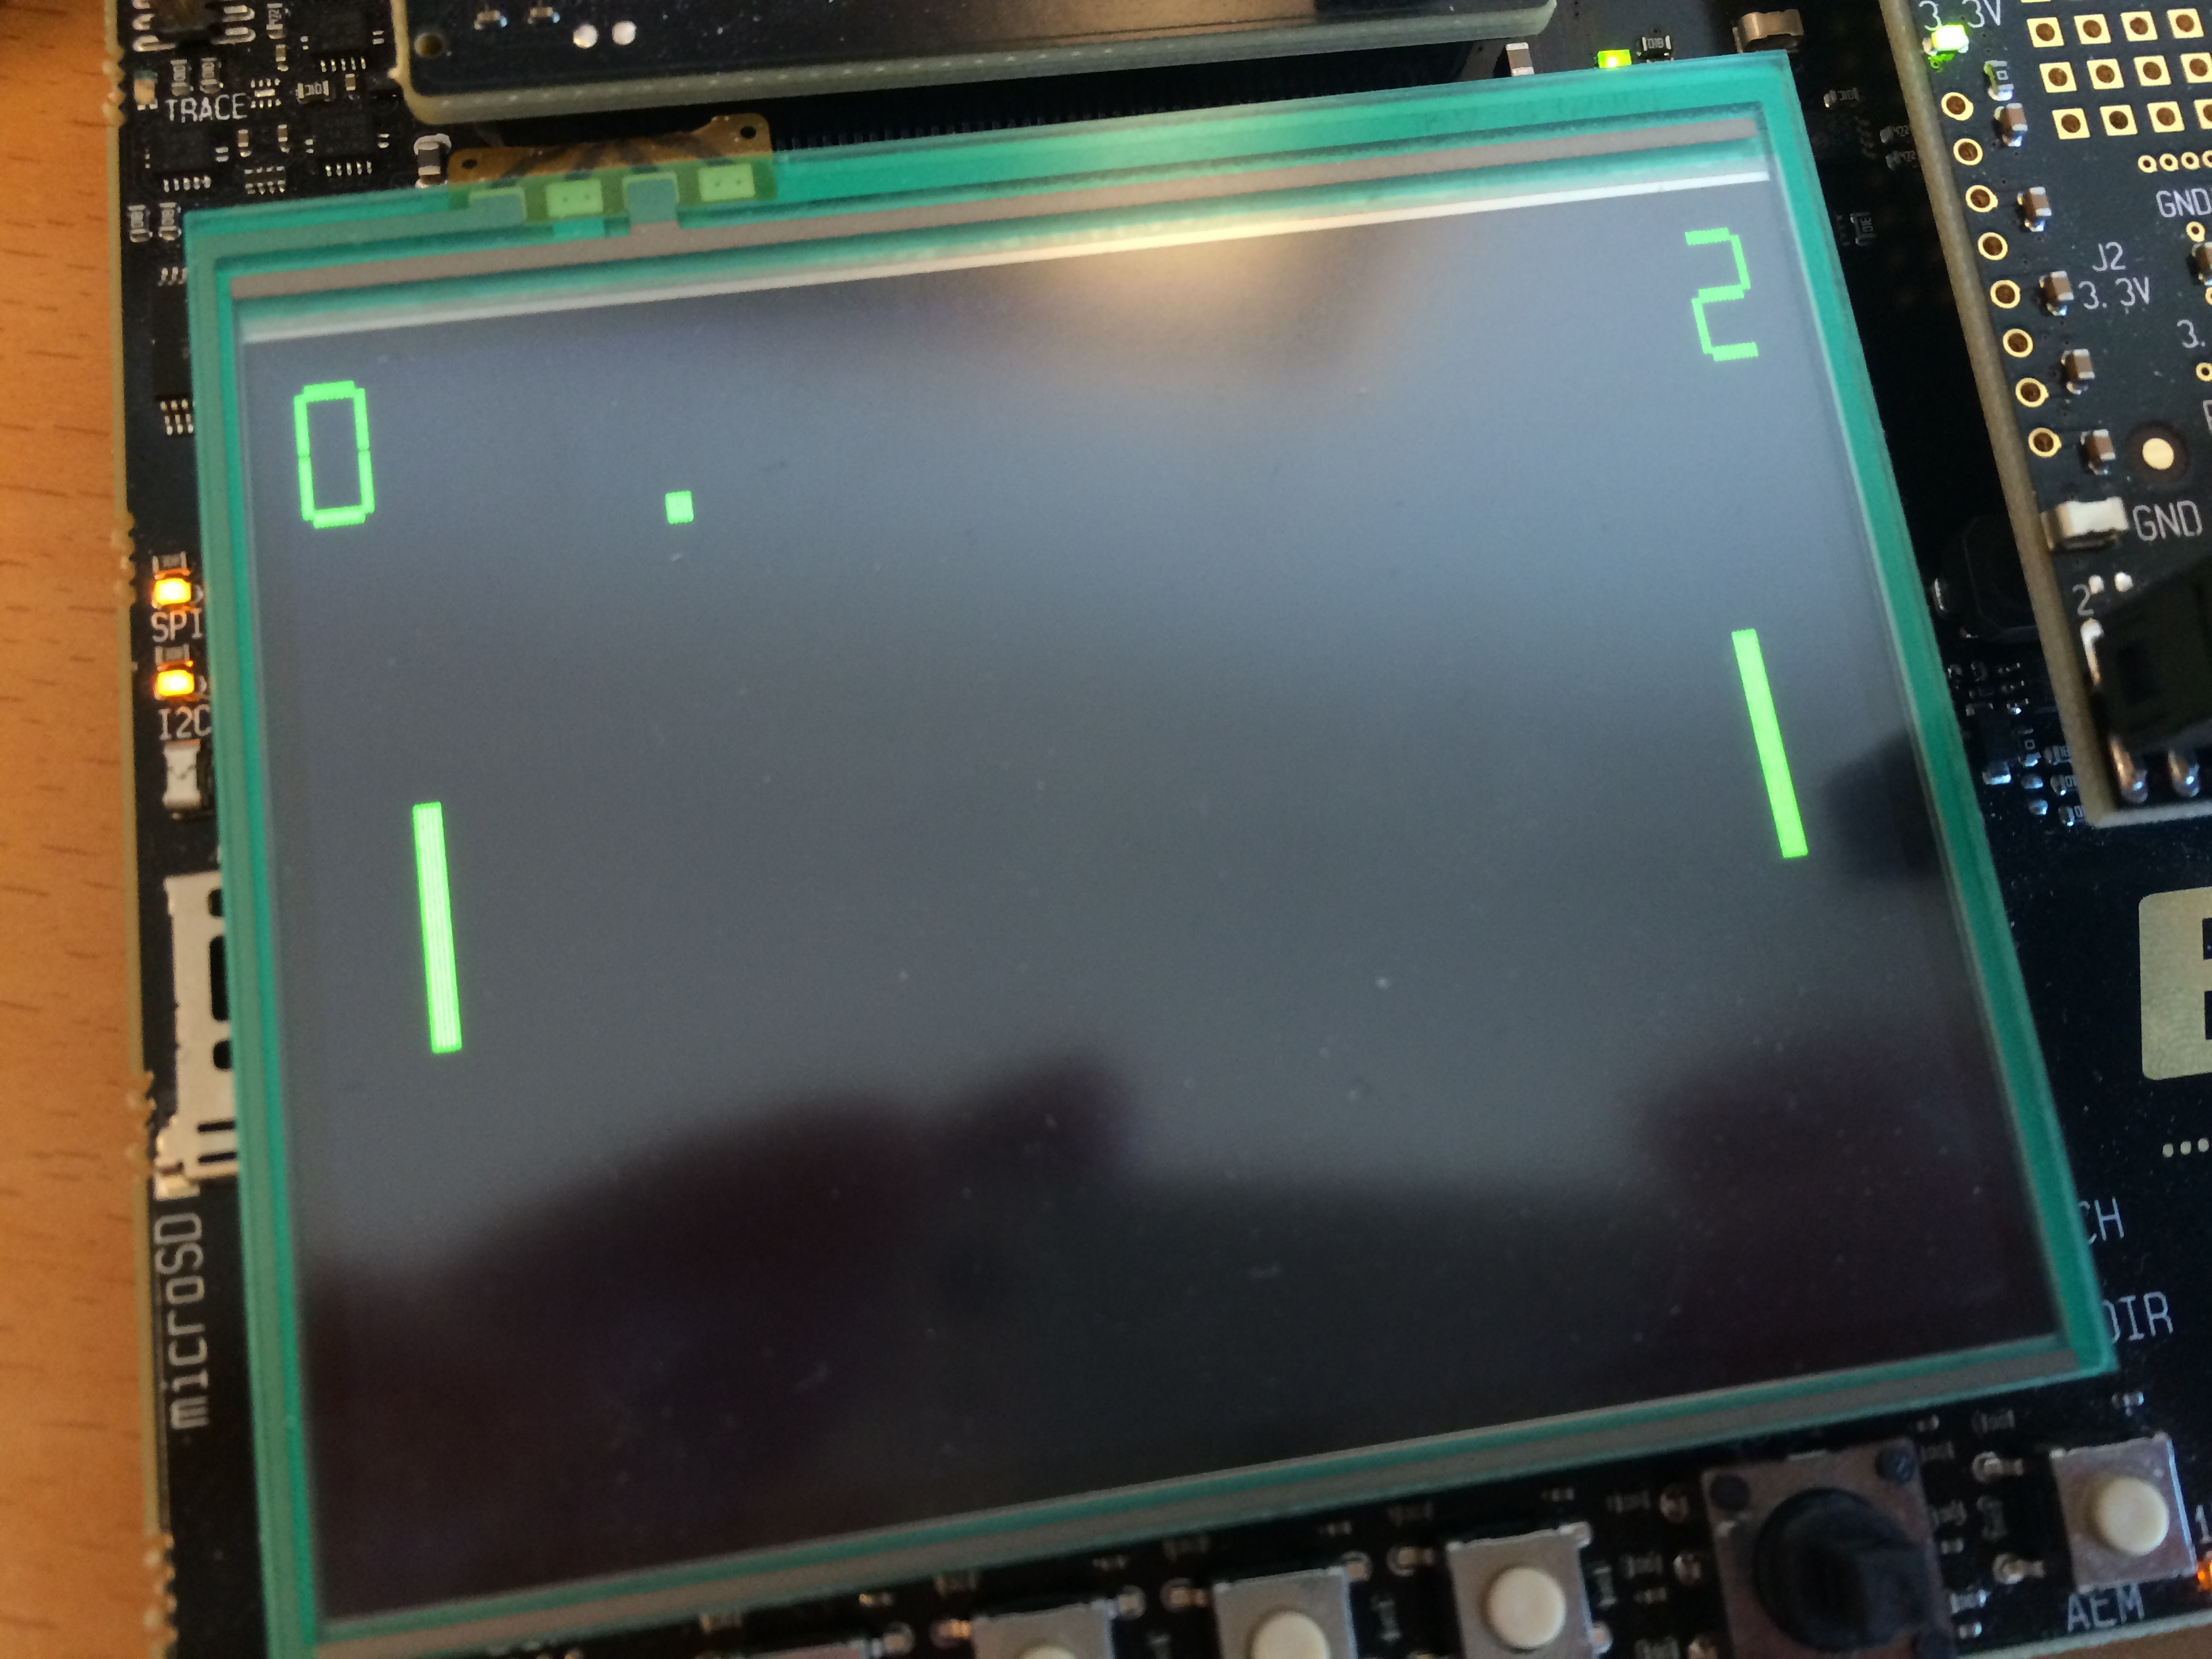
\includegraphics[width=0.8\textwidth]{figures/gameplay.jpg}
\caption{Gameplay shot}

\end{figure}

\subsubsection{Structure of the game}

Following established patterns of game programming, updates of the games
internal state are fully decoupled from the rendering thereof.

At the start of each iteration of the game loop, lag (how much time we haven't
accounted for) is calculated, and caught up with.  This allows the game to
simulate at a fixed rate even on slower hardware, reducing only visual
performance.

If the game loop finishes ahead of time (using less than MS\_PER\_UPDATE ms),
sleep mode is entered for the remainder (time\_to\_next\_update).

With an internal update frequency target of 24 fps, ENTER EXAMPLE WITH
MICROCONTROLLER DATA HERE.  This allows the program to spend most of its time
sleeping.

\begin{algorithm}
  \caption{Game main loop}
  \begin{algorithmic}
    \State $lag \gets 0$
    \State $time\_previous \gets \Call{get\_time}{\null}$

    \Loop
      \State $time\_current \gets \Call{get\_time}{\null}$
      \State $time\_elapsed \gets time\_current - time\_previous$
      \State $lag \gets lag + time\_elapsed$

      \While{$lag \geq MS\_PER\_UPDATE$}
        \State $\Call{update}{\null}$
        \State $lag \gets lag - MS\_PER\_UPDATE$
      \EndWhile
      \State $\Call{draw\_game}{\null}$
      \State $\Call{sleep}{MS\_PER\_UPDATE - lag}$
    \EndLoop
  \end{algorithmic}
\end{algorithm}

\subsubsection{Input handling}
Whenever the gamepad changes state, i.e. a button is released or pressed,
a signal is received which in turn invokes an input interrupt handler.

The handler polls the gamepad driver, receiving a byte representing currently
pressed buttons. Input is then parsed to fit the games internal representation
of active keys. This abstraction layer between input and internal state is used
to allow for multiple methods of input, practical during development when a
computer keyboard is used.

Having an allways up to date version of button state cached frees the program
from having to poll the driver for each iteration of the main game loop.

\subsubsection{Graphics}
To display graphics on the screen, the game uses the Linux framebuffer device.
All the functions for initialising and adding graphics to the framebuffer are
contained in graphics.s.

The initializing function opens the framebuffer file in Linux, and then maps the
file to a region in memory. This is done as it is easier to access an array in memory
than to search back and forth in a file.

As a write to the memory mapped area does not update the framebuffer,
one has to refresh it explicitly.
This is done by sending a special signal to the framebuffer
along with bounding indexes, allowing for partial screen updates.

To actually make graphics,
the draw\_pixel() function is used to fill a given pixel with some color.
It can be called on a subsequent sequence of pixels to create more complex graphics,
e.g. squares and circles.

To get that nice retro look, all geometry in this impementation of pong is rectangular,
set to the color of H4CK3R\_GR33N (The Matrix-green).
It would, however, not be a problem to create other shapes or colors as
all graphics code is generic and nicely abstracted.

\subsubsection{Energy efficiency optimization}
